\ifx \globalmark \undefined %% This is default.
	\input{../header}
\begin{document} %% Crashes if put after (one of the many mysteries of LaTeX?).
\else

\fi



\chapter*{Intro}
\label{chap:intro}

Since the birth of humanity,
Mathematics have been the central tool for scientists and engineers.
Arguably, Mathematics have not only been a language to express concepts
and techniques developed in the different scientific fields,
but it has been very often a key motor of the development of these fields,
thriving on, and at the same time fertilizing the scientific discipline in question.
This is strikingly the case in decision and game theory.

To the best of our knowledge, the formulation of a mathematical Science of Decision Making materialized only in the latter half of the 20th century\footnote{Although, there are notes on the topic dating from the 18th century, written by no other than Daniel Bernouilli.}
That was also the time when computers were invented. That century was marked by two World Wars and the related technological races that ensued.
Scientific and technological discoveries were fueled by those conflicts.
Of particular interest to us, there was a need to optimize the use of resources,
and to make efficient decisions at a scale that was beyond what's capable for the human mind.
``\emph{Beautiful minds}'' like John Von Neumann, or John Nash, where instrumental in the developments that followed.

\paragraph{What is a decision?}
A decision, in its essence,
involves choosing one option from a set of possibilities.
Whether a student selecting courses for a semester,
a restaurant's guest picking a dish from a menu,
or a generative model like ChatGPT adding a word to a sentence,
decisions are omnipresent.

\paragraph{We are interested in a systematic, mathematical study of decision-making.}
The decision-making process is ubiquitous in our daily life. It's study is central to many disciplines,
including Psychology (almost by definition), Economics and Social Sciences.
It is also a key topic in Computer Science, where it is studied in the context of Artificial Intelligence.

Why are some decisions made instead of others? Can they be improved? How could we evaluate the quality of a decision?
These questions form the crux of our scientific inquiry.
The diverse disciplines mentioned above approach them with varying methodologies.

In this course, we will look at them through an abstract, mathematical lens.
We will approach the topic of Decision Theory in itself, where we study single agents making decisions, as a fundation.
Then, we will spend most of our time of Game Theory. To oversimplify, Game Theory is the study of Decision Theory in a multi-agent setting.

\subsection*{Structure}

The contents are divided into 10 chapters. 
The dependencies between chapters are illustrated in Figure \ref{course-map}.

\begin{figure}[!ht]
\centering
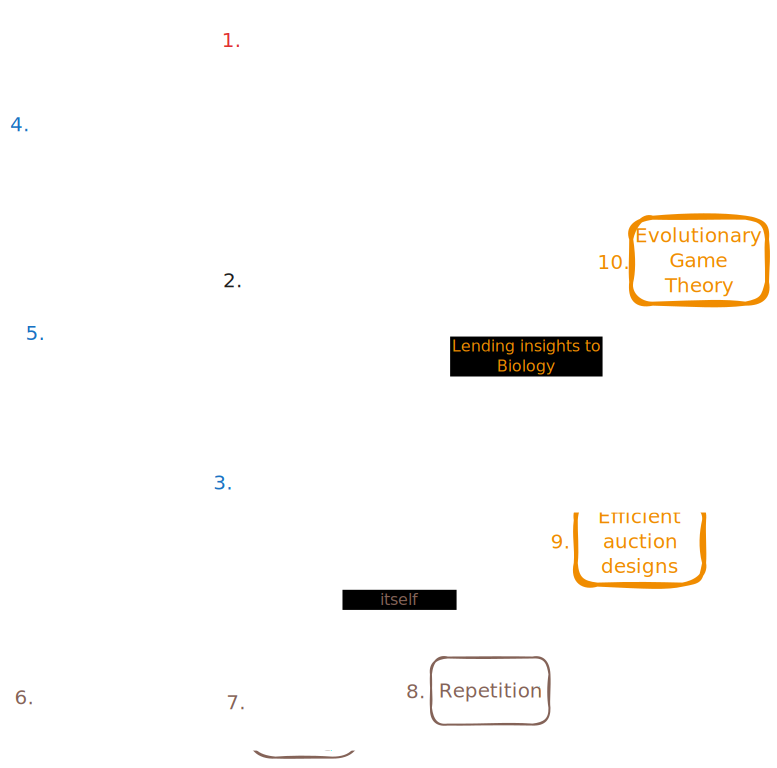
\includegraphics[scale=0.5]{map.png}
\caption{Players must chose rationally if they follow the recommendations of the mediator.}
\label{course-map}
\end{figure}


Notice that the chapters are not necessarily ordered by difficulty, nor by dependency: for instance, Chapter 5 is not a prerequisite for Chapter 9.
Nonetheless, if you are approaching the material through those notes, we recommend to follow the order of the chapters:

\begin{itemize}
   \item Chapter 1: Decision Theory. We start with the fundamental concepts which will capture the behavior of all rational and intelligent agents involved in the course.
   \item Chapter 2: Models of Game Theory. We then explore how to model the interactions between agents as games. There are several options, some are more expressive, some are simpler. 
   		  We also introduce some basic results about those models.
    \item Chapter 3: Nash Equilibrium. We introduce the concept of Nash Equilibrium, which is the most fundamental solution concept in Game Theory -- and arguably the most famous.
    \item Chapter 4: Sequential Games. The more expressive models of games encode temporality. We study the impact of that temporality on the behavior of agents.
    \item Chapter 5: Refinements of Nash Equilibrium. We introduce several solution concepts that sit in between the complex Sequential Equilibrium and the conceptually simpler Nash Equilibrium.
    \item Chapter 6: Games with Communication. We move back to simpler models of games, but we allow agents to communicate before making their decisions, and observe the impact of that communication.
    \item Chapter 7: Bargaining and Coalitions. Somehow orthogonal to the previous chapters, we study the problem of dividing a cake between agents, and the problem of forming coalitions.
    \item Chapter 8: Repeated Games. Some situations are better modeled as a game that is played repeatedly infinitely often. We study the impact of that repetition on the behavior of agents.
    \item Chapter 9: Auctions. A first departure from our formalism of games. We keep the concepts, and apply them to design efficient auctions mechanisms.
    \item Chapter 10: Evolutionary Game Theory. A second departure from our formalism of games. This time, the concepts are borrowed by Biology. We study the evolution of population of agents, adequating the concept of move to that of genome, and nash equilibrium to population equilibrium.
\end{itemize}

Regardless of the order in which you approach the chapters, we recommend to group them in three categories:

\begin{itemize}
	\item Chapter 1 is transversal to the whole course. As a matter of fact, most of the rationale behind the course can be traced back to the concepts introduced in Chapter 1.
	\item Chapters 2 and 3 provide a simple, basic introduction to core concepts in game theory.
	\item Chapters 4 and 5 are more advanced, and explore futher the implications of Chapter 1 in the scope of Chapter 2 and 3.
	\item Chapters 6 to 8 build on the concepts introduced in Chapter 1, 2 and 3, but are more independent from each other.
	\item Finally, Chapters 9 and 10 are more independent from the rest of the course. However, they do require a good understanding of the concepts introduced in Chapters 2 and 3.
\end{itemize}

\subsection*{Thanks from Prof. Rapha\"el Jungers}

These notes are the result of the work of many people.

I want to express my deep gratitude to the several generation of contributors to those notes.
The first edition was contributed by \emph{Romain Hollanders}, \emph{Sebastian Stich}, and \emph{Matthew Philippe}. 
They worked hard on the first versions of these notes. Many pedagogical ideas presented in these notes come from them. 
In particular, I want to stress the amazing work achieved by Matthew, who was leading the project from the first drafts to the final version, not only in writing, but also for many higher level ideas.  Thanks a lot!

In the years following the first edition, many students contributed to the notes, by pointing out typos, or by suggesting improvements, or more naturally, by asking their questions out loud.
We are grateful to all of them. In particular, I want to thank \emph{Benoit Legat} 
for taking over the source code of the notes, and for maintaining it for several years.

Additionally, thanks to our amazing TAs. They are in the front seat, helping us gauge the understanding of the students, and they are the ones who are in the best position to suggest improvements.
Many thanks to \emph{Brieuc Pinon} and \emph{Anne Rubbens}!


\ifx \globalmark \undefined %% This is default.
\bibliographystyle{plain}
\bibliography{../gametheorybibliography}
\end{document}
\else

\fi




